\documentclass[letterpaper,12pt]{article}
\usepackage{graphicx,amsmath,fancyhdr,times,setspace}
\usepackage{upquote,framed}
\oddsidemargin -0in %left margin on odd-numbered pages is 1in + 0in
\topmargin -.5in %top margin is 1in -0.5in
\headheight 15pt

\textwidth 6.375in %width of text
\textheight 9in % size of page
\setlength{\parindent}{0.0in}
\setlength{\parskip}{10pt}
\renewcommand{\thefootnote}{\fnsymbol{footnote}}

\newtheorem{question}{Question}
\usepackage{pdfpages}
\usepackage{url}
\usepackage{caption}

\newcounter{lnum}
\newenvironment{abbrevlist}%
  {\begin{list}{$\bullet$}{\setlength{\leftmargin}{2em}%
               \setlength{\itemindent}{0em}%
               \setlength{\itemsep}{0pt}%
               \setlength{\parsep}{0pt}%
               \setlength{\topsep}{2pt}%
               \usecounter{lnum} } }{\end{list}}


\pagestyle{fancy}
\lhead{MEOPAR Prediction Core Winter School 2017}
\rhead{Regional Models-\thepage}
\chead{ }
\fancyfoot[C]{\tiny Notes for Regional Models by Susan Allen and The University of British Columbia are licensed under a Creative Commons Attribution 3.0 Unported License}

\input{../def}

\begin{document}

\title{MEOPAR Prediction Core Winter School 2017: Regional Models}
\author{Susan E. Allen }
\date{\today}
 \maketitle


\setcounter{tocdepth}{3}

\setlength{\parskip}{0ex}


\section{Learning Goals}

By the end of this module, students will be able to:

\begin{abbrevlist}
\item describe regional models, their purposes and some of their unique issues
\item analyze the scale dependence of a parametrization
\item discuss the input fields needed to force various types of models
\end{abbrevlist}

\section{Class Time Structure}

\begin{abbrevlist}
\item {\bf Mini-Lecture} Regional Models, Uses and Issues
\item {\bf Worksheet} Determine the scale dependence of a bottom boundary layer
\item {\bf Discussion} Forcing fields for Regional Models
\end{abbrevlist}

\section{Regional Models, Uses and Issues}

\subsection{What is a Regional Model?}

A regional model is a model that only explicitly models part of the whole domain (Figure~\ref{plt:examples}).  In the atmosphere circulation, ocean circulation, and ocean wave models that would a less-than global model.  The implication is, to a lesser or greater extent, the un-modelled part impacts the region explicitly modelled.  Inherently regional models have open boundaries.  We will come back in detail to that issue in the laboratory this evening.

\begin{figure}[h]
\noindent\resizebox{0.3\textwidth}{!}{\includegraphics{../MeoPar/private-docs/presentations/Stakeholders2016/poster/domain_bathy.png}}
\resizebox{0.38\textwidth}{!}{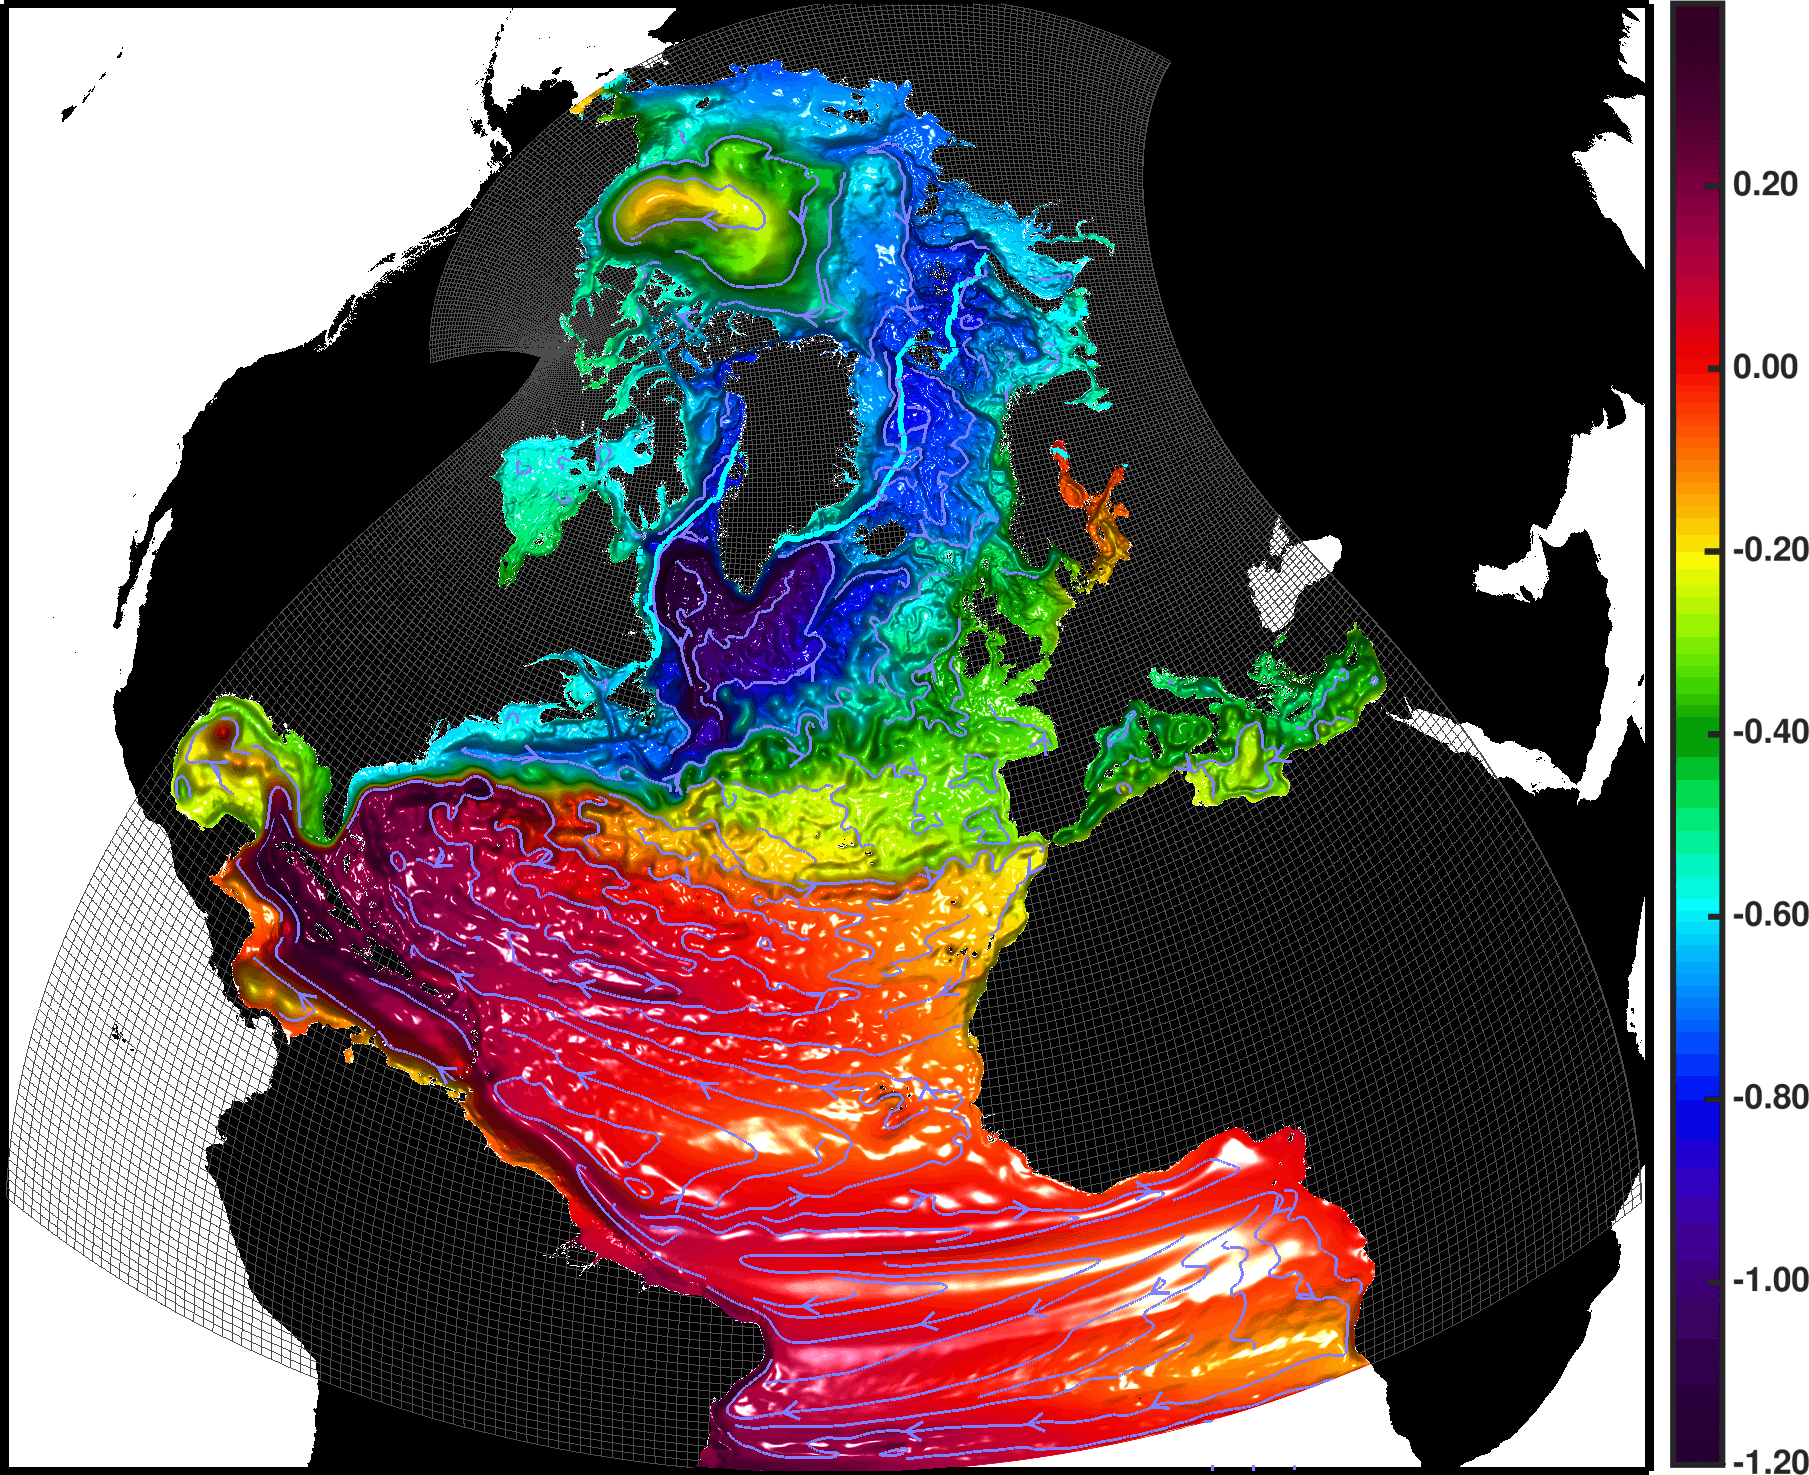
\includegraphics{anha_ssh.png}}
\resizebox{0.3\textwidth}{!}{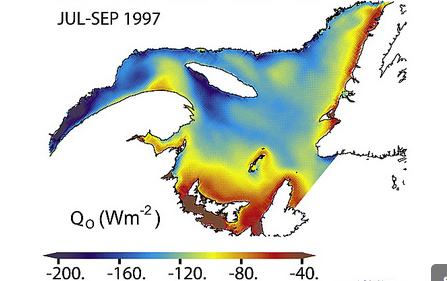
\includegraphics{saucier.png}}
\caption{\protect\it{\small Examples of Canadian Regional Ocean Models: SalishSeaCast (UBC), ANHA4 (UAlberta), Gulf of St. Lawerence (MLI, DFO)}}
\label{plt:examples}
\end{figure}
  
\subsection{What are Regional Models Used For?}

In science, models in the broadest sense are used for many purposes including: to conceptualize our thinking; to quantify conceptual processes; to investigate nonlinearity, multi-processes and other complexities.  They are also used to hindcast or to predict realistic fields for ``downstream'' processes such as response planning or policy.

Regional models can be used as ``process'' models or as ``realistic'' models.  In the former, we simplify and isolate to understand the key processes.  In the latter, we include all necessary processes to reach our goal of accuracy.  Note that both of these require choices.  Choices in what to include and in what to leave out.

Process model often inform parametrizations that are later incorporated into realistic models.

Examples of Process Models:
\begin{abbrevlist}
\item Single submarine canyon study to determine upwelling scaling
\item Zooplankton aggregation in a flow over a ridge
\end{abbrevlist}

Examples of Realistic Models:
\begin{abbrevlist}
\item One-dimensional model for the timing of the spring phytoplankton bloom
\item Storm surge prediction model
\end{abbrevlist}

\begin{figure}[h]
\noindent\resizebox{0.5\textwidth}{!}{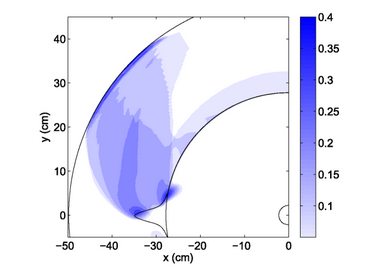
\includegraphics{howattallen.png}}
\noindent\resizebox{0.5\textwidth}{!}{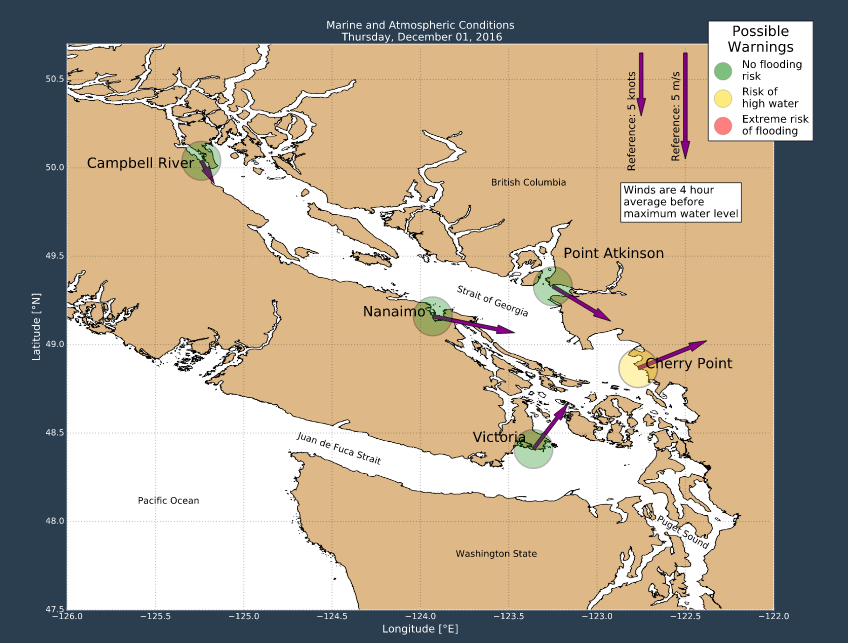
\includegraphics{salishseacast01dec16.png}}
\label{plt:processrealistic}
\caption{\protect\it{\small Left: Process Model: upwelled water for a single canyon (Howatt and Allen, 2013) Right: Realistic Model: storm surge prediction (SalishSeaCast)}}
\end{figure}

\subsection{What Modelling Frameworks are Used for Regional Models?}

Examples include:
\begin{abbrevlist}
\item Regional Ocean Model System
\item FVCOM
\item Weather Research and Forecasting Model
\item MITgcm
\item NEMO
\item WW3
\item GEM
\end{abbrevlist}

All these model frameworks can be used for process or realistic modelling.

The first three models were designed as regional models. The other models were designed as global models but are used in regional configurations as well.

\subsection{What are some of the special issues with Regional Models?}

Open boundaries are common to all regional models.  For this section though, I want to focus on coastal models.

\subsubsection*{What is different about the coastal ocean than the global ocean?}

\begin{abbrevlist}
\item Shorter time and space scales
\item Shallower water
\item Complicated coastlines matter
\item Complicated topography matters
\item Faster flows
\item Tides usually must be included
\item Interactions with the land: freshwater
\item Usually stronger mixing
\end{abbrevlist} 

\subsubsection*{How does that impact our models?}

\begin{abbrevlist}
\item Smaller grid scales, smaller time steps, shorter runs
\item We want finer horizontal resolution to follow the topography (unstructured grids?)
\item Better topography resolution (vertical grid choices)
\item Vertical velocities can be significant.
\item Flow might not be hydrostatic!
\item Need to include freshwater
\item Background numerical diffusion is less of an issue
\end{abbrevlist}

\subsubsection*{Numerical Diffusion}

Most numerical models have inherent numerical diffusion.  That is,
even if you set the molecular and turbulent diffusivities to zero,
sharp gradients in salinity, temperature, nitrate etc, still diffuse with time.  This process occurs both in the vertical and horizontal.  Usually the advection schemes are the culprit as it is hard to keep advection stable without some diffusion.  Different models have different levels of inherent diffusion.

In the deep open ocean, for climatological time scales in particular, natural diffusion is slow and numerical diffusion can be significant.  Schemes to ensure that strong isopycnal diffusion does not contaminate slow diapycnal diffusion are common.  In the coast ocean, a key feature is the strong halocline below freshwater which can also be subject to too strong diffusion.

\subsubsection*{Structured versus Unstructured Grids}

Unstructured grids can beautifully follow complicated coastlines (Figure~\ref{plt:unstructured}).  They can resolve bays and channels and the telescope out so that areas of less interest or less complication have large cells and thus take less computational effort.

\begin{figure}[h]
\noindent\resizebox{0.5\textwidth}{!}{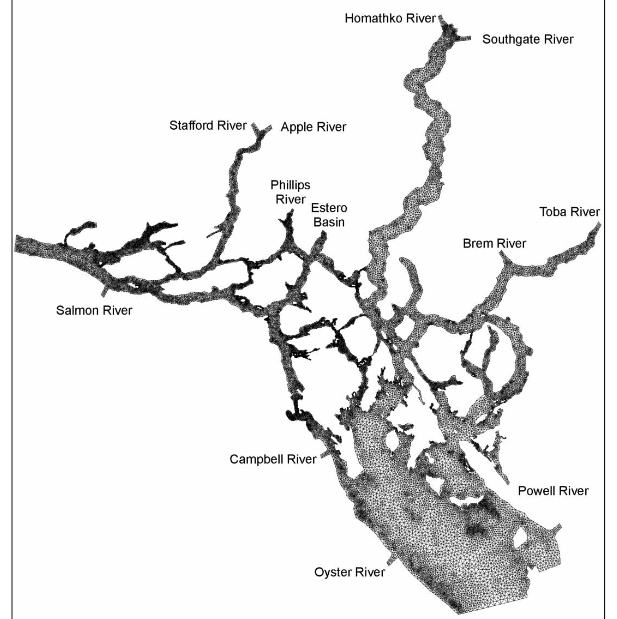
\includegraphics{foreman2012.png}}
\resizebox{0.5\textwidth}{!}{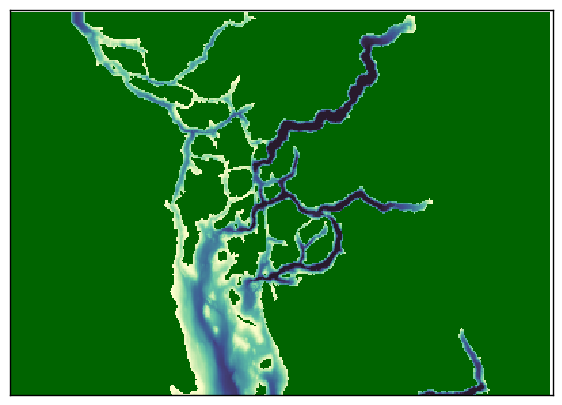
\includegraphics{SalishSeaCastDiscovery.png}}
\caption{\protect\it{\small Discovery Islands in Left: Foreman et al
    (2012)'s unstructured FVCOM model and Right: SalishSeaCast's structured NEMO model}}
\label{plt:unstructured}
\end{figure}

On the negative, they can be quite diffusive: you can lose your nice sharp halocline with weeks.  The problem is that the unstructured grid makes using higher order advection schemes (that are less diffusive) difficult.  They can also be computational expensive in comparison to structured grids.  Note that structured grids can be gently bent to match large scale coastline curves.

\subsubsection*{Topography}

Topography is a bigger percentage of the total water depth (up to
100\%) in the coastal ocean.  Its resolution and treatment is critical
across a range of processes.  Various types of vertical coordinates
are possible (Figure~\ref{plt:nemobook}) including isopycnal layers
(not shown).  The type of vertical coordinate determines how the topography is resolved.

 \begin{figure}[h]
\resizebox{0.7\textwidth}{!}{\includegraphics{madecNEMObook.png}}
\caption{\protect\it{\small A range of different vertical grids available in NEMO (Madec et al, 2016)}}
\label{plt:nemobook}
\end{figure}

For gentle slopes, terrain-following coordinates also called sigma
coordinates (Figure~\ref{plt:nemobook}c) have show very good success.
There is a difficulty of two many levels in shallow water that a mixed
coordinate can alleviate (Figure~\ref{plt:nemobook}d, e).

Terrain following coordinates can generate spurious flows due to pressure gradient and vertical velocity errors.  These errors are reduced by smoothing the topography.

I prefer z-coordinate grids with partial steps (Figure~\ref{plt:nemobook}b) for two reasons.  My region (and in particular my interests) are over steep topography and too much smoothing changes the dynamics.  There are problems with the steps of a z-coordinate model but my intuition is much better on flow over steps than some of the artifacts of sigma-coordinate models.

\subsubsection*{Vertical Velocities}

Steep topography and strong coastal tides lead to large vertical velocities.  Many models assume the pressure is hydrostatic (equal to the weight of water above plus atmospheric pressure).  That means that in this equation:

\begin{equation}
\dwdt + u \dwdx + v \dwdy + w \dwdz = - \frac 1 {\rho_o} \dpdz - \rho^{\prime} g + {\rm turbulent viscosity}
\end{equation}

the largest terms by far are the first two on the right side of the equation.  You can check this in two ways: scale the equation for your regional model or run a non-hydrostatic model and see if there is a difference.  MITgcm has a non-hydrostatic choice.  So far we have only seen differences in internal waves, not in the mean flow we study over canyons.

Even though vertical velocity is neglected in the momentum equations, vertical advection is a key component of all the tracer equations.  Strong vertical velocities and fine vertical resolution can lead to instability (CFL) in explicit schemes.

\subsection{How do you Choose a Model Framework?}

Model choice and configuration will always be a compromise.  There are funders preferences, what is well documented and easy to use, what the rest of your institute is using.  

However, it is important to think about:
\begin{abbrevlist}
\item your {\bf Research Questions} 
\item the key {\bf Processes} in your region and what it will take to model those well
\item processes that are important elsewhere that are not key in your region
\end{abbrevlist}

\begin{figure}[h]
\noindent\resizebox{0.5\textwidth}{!}{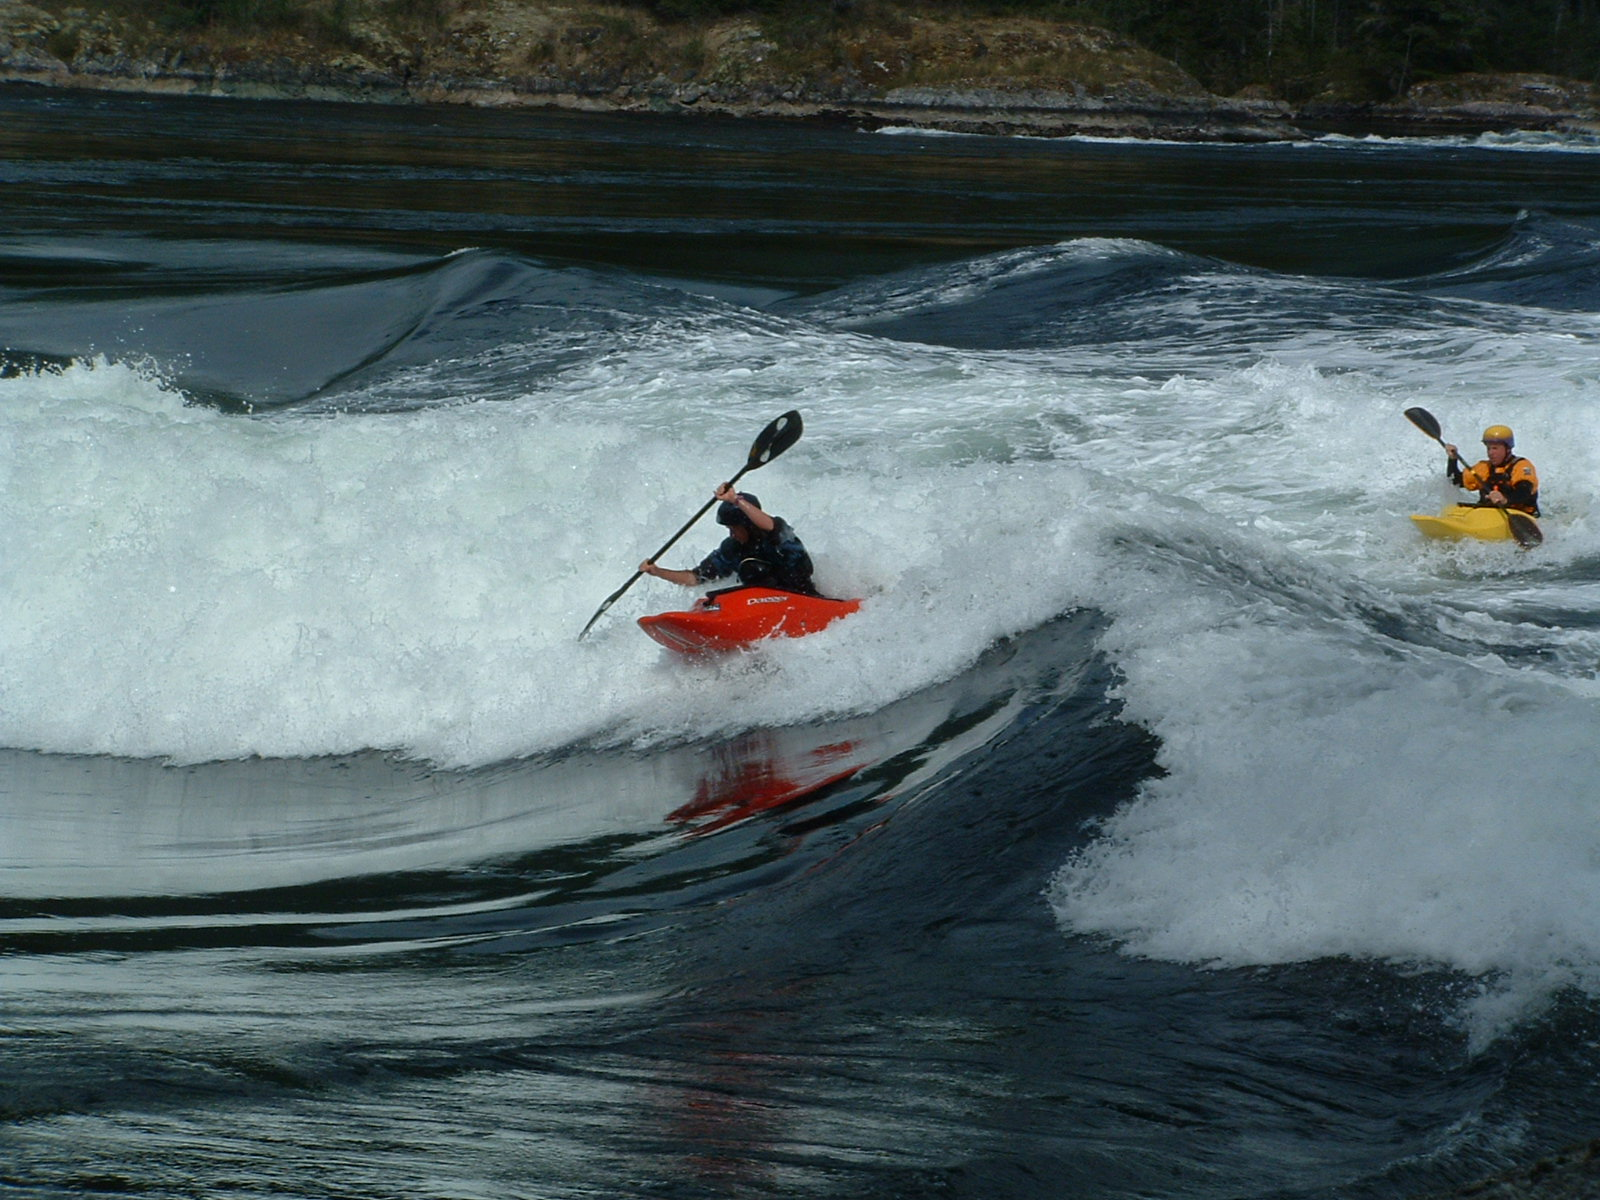
\includegraphics{jthorlacius.jpg}}
\resizebox{0.5\textwidth}{!}{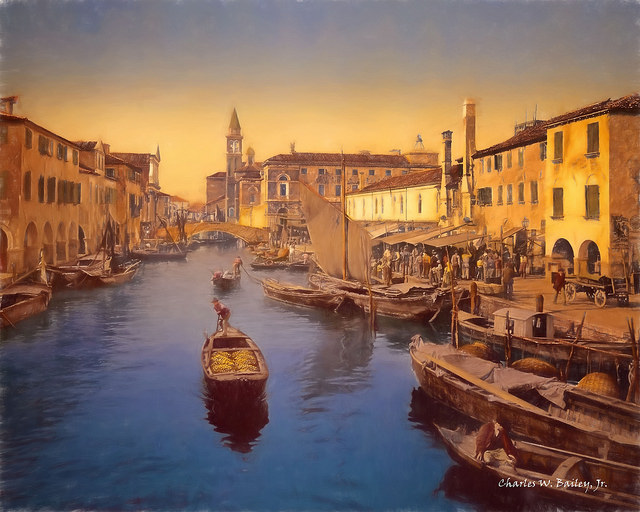
\includegraphics{16122583090_550b93988b_z.jpg}}
\caption{\protect\it{\small Skookumchuk Rapids (by J. Thorlacius) and Chioggia, Italy (by Charles Bailey)}}
\label{plt:contrasts}
\end{figure}

\clearpage

\section{Worksheet}


{\bf\large Names:}


\subsection*{Scale Dependent Parametrizations}

Consider a steady flow of 10 cm s$^{-1}$ over a flat bottom in a turbulent ocean.  We will neglect impacts of stratification and rotation.  In a large scale ocean model we would parametrize the drag of the bottom using an nonlinear, quadratic drag law of the form:

\begin{equation}
\tau = C_D \rho u^2
\label{eq:drag}
\end{equation}
where $\tau$ is bottom drag or stress, $\rho \approx 1000$ kg m$^{-3}$ is the density of water, $u$ is the flow speed above the bottom and $C_D$ is the drag coefficient.  The drag coefficient is a bit of a fudge factor and depends on your problem.  Here we will use 0.01.  In SalishSeaCast I tune it to get the tides accurate.

\begin{question}
What is the drag? \\
$\tau = $\\[24pt]
\end{question}

Let's look a little closer, below is a grid diagram
(Figure~\ref{plt:grid}).  Given the flow of 10 cm s$^{^-1}$ at the
lowest grid cell $u_1$, the drag on that velocity is the value given above.

\begin{figure}[h]
\resizebox{3in}{!}{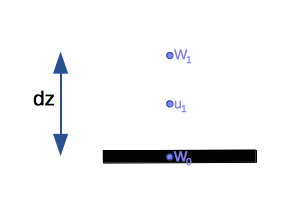
\includegraphics{grid.png}}
\caption{\protect\it{Typical grid near the bottom. $w$ is the vertical
    velocity, the black line is the bottom. No flow through the bottom
    implies $w_0 = 0$.} Lowest horizontal velocity grid point $u_1$ is
  $dz/2$ from the bottom.}
\label{plt:grid}
\end{figure}

\clearpage

In the ``real world'' we would expect a log layer profile (Figure~\ref{plt:loglayer}):

\begin{equation}
u = \max \left[ \frac {u_*}{\kappa} \log \left( \frac z z_* \right), U \right]
\end{equation}
where $u_* = (\tau/\rho)^{1/2}$ is the friction velocity, $\kappa =
0.41$ is von Karman's constant, $z$ is height above the bottom, $z_*$
is the roughness length, here 20 cm, and $U$ is the free stream (above boundary layer) velocity.

\begin{figure}[ht]
\resizebox{5.5in}{!}{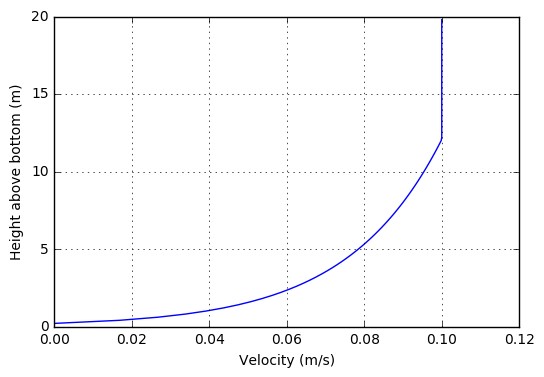
\includegraphics{loglayer.png}}
\caption{\protect\it{Log layer velocity profile.}}
\label{plt:loglayer}
\end{figure}

To match the log-layer to the bottom stress parametrization above we
find that 
\begin{equation}
u_* = \frac U {C_D^{1/2}}
\end{equation}

Let's assume that the model velocity at each grid point is exactly the log
layer value at the appropriate height above the bottom.  That is, you can
find $u_1$ from Figure~\ref{plt:loglayer} by reading off the graph the
value at $dz/2$.

For a large scale model a  typical bottom layer box thickness, $dz =
30$~m.  In coastal models we usually have better resolution.  What
happens if we use the parametrization (\ref{eq:drag}) but have better resolution?

\clearpage

\begin{question}
What is the drag using the quadratic drag law  (\ref{eq:drag}) for the
flow shown in Figure~\ref{plt:loglayer} for bottom grid resolutions of
$dz = $10, 5 and 2 m?\\
With $dz=10$m , $\tau  = $\\[24pt]
With $dz=5$m , $\tau  = $\\[24pt]
With $dz=2$m , $\tau  = $\\[12pt]
\end{question}

\begin{question}
Should the drag change in this way? Why or why not?
\end{question}

\vspace{1in}

\begin{question}
Noting that our bottom grid cells are not always the same size, in
shallower water they are often smaller, how should we parametrize the
bottom drag?\\[24pt]
\end{question}

\clearpage

\section{Forcing Fields for Regional Models}

\begin{abbrevlist}
\item What types of forcing do you need?
\item For what time period?
\item With what spatial and temporal resolution? 
\end{abbrevlist}

\subsection*{Atmospheric}

\begin{abbrevlist}
\item Winds
\item Precipitation : amount and type
\item Solar radiation, Long wave radiation
\item Humidity (or latent heat flux)
\item Temperature (or sensible heat flux)
\end{abbrevlist}

\subsection*{Land}

\begin{abbrevlist}
\item Run off, rivers
\item Groundwater seaps
\item Temperature of this water
\item Tracers in this water
\end{abbrevlist}

\subsection*{Bottom}

\begin{abbrevlist}
\item Geothermal heat flux
\item Tracer exchange with sediments
\end{abbrevlist}

\subsection*{Open Boundaries}

\begin{abbrevlist}
\item Currents -- perhaps split between barotropic and baroclinic
\item Tides -- sea surface height and currents
\item Sea Surface Height
\item Temperature, Salinity and other tracers
\item Ice
\item Waves
\end{abbrevlist}

\subsection*{Sources}

\begin{abbrevlist}
\item Simple analytic expressions, constants or time series estimated from data or previous models
\item Climatologies 
\item Data
\item Other models
\end{abbrevlist}

\subsection*{How ``good'' is your forcing?}

Don't neglect evaluating your forcing for your use!

\end{document}